\documentclass{article}
\usepackage[utf8]{inputenc}
\usepackage{amsmath,amssymb} 
\usepackage{graphicx}
\usepackage{enumitem}
\usepackage{multirow}
\usepackage{hyperref}
\usepackage{url}

\title{CS677 Assignment \#1}
\author{Aayushi Verma (\#U01865004)}
\date{due 7/2/23}

\begin{document}

\maketitle
% template image: \includegraphics[scale=0.1]{hw5_q2_1.jpg}
% template list: \begin{enumerate}
%    \item blah
%\end{enumerate}
% template code: \begin{verbatim}
%    code
%\end{verbatim}

\section{Question One}
\noindent \textbf{Create a graph showing the number of hours studied and the grades earned using the below information (Take hours on X-axis and grades on Y-axis). Describe how studying hours affect grades.}

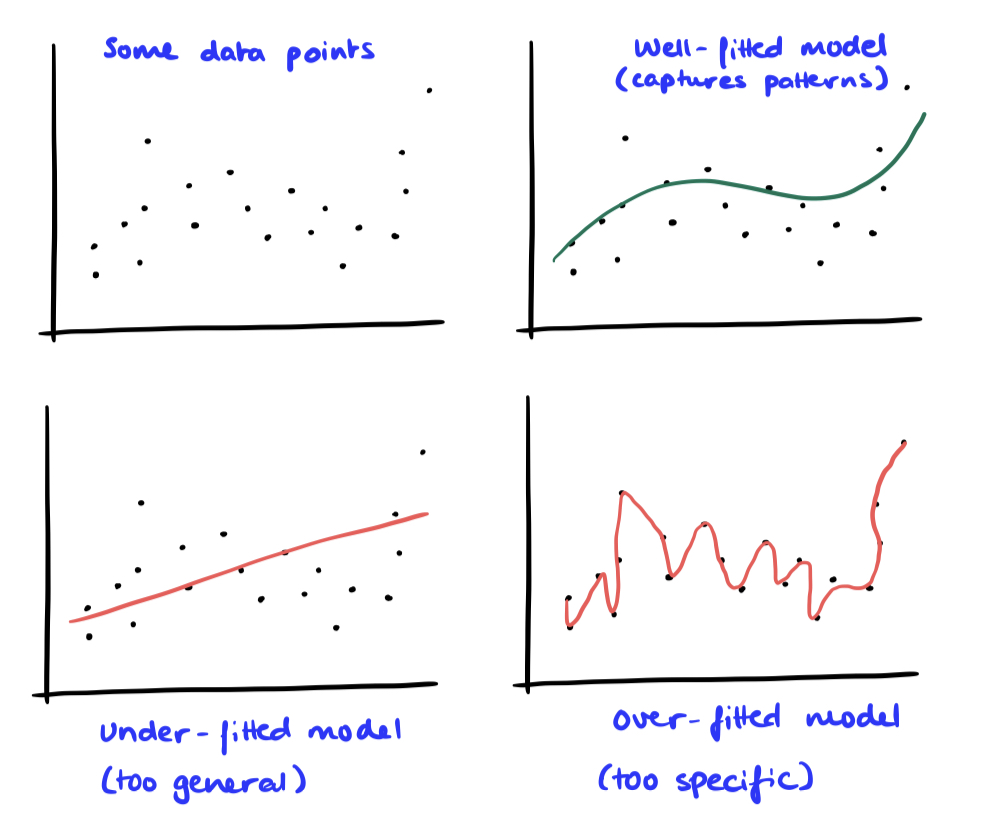
\includegraphics[scale=0.3]{q1.png}

We see that there is a general positive trend, i.e. as the number of hours studies increases, the grade points achieved also generally increases.

\section{Question Two}
\noindent \textbf{[Credit-worthiness assessment] - Predict the probability of a customer being a potential defaulter based on past transaction data and historical information about customers who have defaulted/not defaulted in their payments.}
\newline

\noindent \textbf{(i) What type of Machine Learning does this problem belong to? How?}

This is an example of a binary classification problem, i.e. supervised learning. This is because there are two classes we want to classify the prediction of customer data as either defaulter or non-defaulter.
\newline

\noindent \textbf{(ii) Referring to the Week 1 topic Formal Learning stages (slides 17-21), list all the steps required to implement the ML solution. (ML algorithm name
not required)}

The solution can be implemented by the formal learning process.

Stage One  of the process is identifying the inputs and outputs of the learning process. This includes having:
\begin{enumerate}
    \item Data instances, in this case collection of customer historical transaction data categorized as defaulter or non-defaulter
    \item Features (attributes) of the data. Some examples of possible features for this dataset might include customer demographics (age, race, gender, etc.), credit score, tenure with vendor, mortgages, etc.
    \item Labels, which in this case are: defaulter, or non-defaulter.
\end{enumerate}

Stage Two of the process is training the data. The dataset should be large enough to cover a variety of hypotheses to build a reasonable model. It should also not have too much noise to build a reasonable model.

Stage Three of the process is splitting the dataset into training samples, validation samples, and testing samples. These three subsets of the dataset must be distinct from each other, and each serve a certain purpose.
\begin{enumerate}
    \item Training data is for building and training the model. 
    \item Validation data is for validating the quality of the model's learning. 
    \item Testing data is for testing the performance of the model.
\end{enumerate}

Stage Four of the process is evaluating the model. This is done using the following:
\begin{enumerate}
    \item Loss function - function which measures the difference between the actual label in the test dataset and the predicted label returned by the model.
    \item Hypothesis set - a set of parametric functions which determine the hypothesis used by the model, i.e. what features contributed to the predictions, and their associated accuracies.
\end{enumerate}
\newline

\noindent \textbf{(iii) If your ML solution doesn't perform as expected, what do you think might be the reason? Any ideas about how to deal with a model like that?}

As detailed in my answer in (ii), there are several points in the learning process which can be re-evaluated in case the ML solution doesn't perform as expected. 

In Stage One, we can check if the dataset has enough features and is of a good size. If the dataset is too small or doesn't have enough features, the model will learn only from that limited dataset, and won't perform well on a larger dataset or on a dataset with more features. Also, it is important to choose an algorithm that solves the problem the dataset constitutes, i.e. if the dataset has labels for defaulter or non-defaulter, then it does not make sense to choose e.g. a regression problem, because that is unsuited to the dataset.

In Stage Two, we can check if the dataset has a lot of noise. In other words, if the dataset is not clean and unrepresentative of the problem, then the model will not perform well when applied to a test dataset. The relevance of features should also be considered, i.e. if there are any features that do not add value to the problem, then those may just be noise and should be removed.

In Stage Three, we can check if the dataset was split appropriately into training, validation and test samples. Generally, the training/test split is usually like 70/30 or 80/20. The split should be neither underbalanced nor overbalanced. The validation split should also be taken into consideration.

In Stage Four, the hypothesis set can be reconsidered if there are certain features that contribute heavily, or do not contribute at all, to the model's predictions. 

%\newline

\section{Question Three}
\noindent \textbf{Give four examples of clustering (different from the ones given in slides) and mention when it is useful.}

Clustering is an unsupervised machine learning technique that clusters or groups data points together that are similar to each other. Some examples of clustering applications I have read about include:

\begin{enumerate}
    \item Identifying fake news - this example uses textual data and identifies bodies of text that contain fake news based on the clusters of words in the text. This application is useful for identifying articles that contain fake news or promote mis/disinformation.
    \item Species identification - this example uses numerical data on species and groups together different populations within the species based on shared characteristics. This application is useful for identifying sub-populations within species and determining the characteristics that differ.
    \item Sport team clustering - this example uses numerical data on sport team members to identify groups of the best and worst players. This application is useful for sport team managers to give individualized training to their players, or for sports fans for betting, for example.
    \item Insurance customer identification - this example uses numerical data on customers on insurance plans and groups similar customer profiles together. This application is useful for identifying groups of customers who would be suited for certain insurance plans.
\end{enumerate}

\section{Question Four}
\noindent \textbf{What are the names of the two loss functions $L_s$ and $L_D$ that we discussed in Week \#2 class time? Explain in detail with examples. What is the topic connecting these two loss functions and give the equation for the same? (Your answer must be at least 150 words)}

$L_S$ is empirical loss, and $L_D$ is true loss. The concept that connects these two losses is learning via uniform convergence, and more broadly, empirical risk minimization. Below follows a detailed explanation.

A predictor is developed by the machine learning algorithm during the training phase, and is a function that takes as input a set of parameters, $\Theta$, and outputs a predicted label, $\hat{y}$ for a data point. Predictors are used during the machine learning process to learn from the training set of data, develop rules and inferences for labeling an unseen data point, and testing the performance of the predictor on unseen test data points, i.e. the predictor makes a prediction, $\hat{y}$, which is then compared against the true label, $y$, using a loss function. The loss function quantifies how approximate the predicted label $\hat{y}$ is to the true label $y$.

The machine learning process receives as input a training sample of data, $S$, which is sampled from an unknown distribution $D$. Given that $D$ is unknown, the true loss cannot be known either. Therefore, in order to approximate a loss, the empirical loss, $L_S$ is calculated as:

\begin{equation}
    L(\Theta) = \frac{\Sigma_{i=1}^{n} l(g_{\Theta}(x)^{i}-y^{i})}{n}
\end{equation}

In other words, the empirical loss is the average loss over the training data points. However, it does not provide an accurate representation of the true loss. The true loss, $L_D$ is determined using the empirical loss predictor, except that the true loss is calculated using the test dataset, and averaged over the test data points. 

In order to have a good predictor, we need to minimize the empirical loss with respect to the training set of data $S$ and with respect to the distribution $D$. For a chosen loss bound, $\epsilon$, if the training sample $S$ has an empirical loss $L_S \leq \frac{\epsilon}{2}$, the Empirical Risk Minimization (ERM) learning rule guarantees to return a good hypothesis. This is called learning via uniform convergence, because the empirical loss is close to the true loss uniformly over all hypotheses. This is also represented as:

\begin{equation}
    L_S (h) - L_D (h) \leq \epsilon
\end{equation}

where $L_S(h)$ is the empirical loss, $L_D(h)$ is the true loss, $\epsilon$ is the chosen loss bound, and for each $h$ in a class $H$, $L_S(h)$ is determined with respect to the training sample $S$, and $L_D(h)$ is determined with respect to the distribution $D$.

\end{document}